% ===================================================================
% tableau_preprocessing_functions.tex — Preprocessing Functions trong Tableau
% Xuất từ tableau_preprocessing_functions.md theo chuẩn AIO2025
% ===================================================================

\documentclass[12pt]{article}

% --- Tiếng Việt ---
\usepackage[utf8]{vietnam}
\usepackage[vietnamese=nohyphenation]{hyphsubst}
\usepackage[vietnamese]{babel}
\AtBeginDocument{\shorthandoff{"}}

% --- Packages cơ bản ---
\usepackage[table,dvipsnames]{xcolor}
\usepackage{booktabs}
\usepackage{ragged2e}
\usepackage{caption}
\usepackage{subcaption}
\usepackage{float}
\usepackage{amsmath,amssymb,amsfonts}
\usepackage{graphicx}
\usepackage{adjustbox}
\usepackage{multicol}
\usepackage[inline,shortlabels]{enumitem}
\usepackage{setspace}
\usepackage{longtable}
\usepackage{titling}
\usepackage{tabularx}
\usepackage{makecell}
\usepackage[T1]{fontenc}
\usepackage{lmodern,mathrsfs}
\usepackage{hyperref}
\usepackage[most]{tcolorbox}
\usepackage{fontawesome5}
\usepackage{listings}
\usepackage{geometry}

\geometry{a4paper, margin=2.5cm}

% --- Màu sắc AIO ---
\definecolor{aivnGreen}{RGB}{0,128,0}
\definecolor{aivnBlue}{RGB}{41,98,255}
\definecolor{aivnOrange}{RGB}{255,152,0}
\definecolor{aivnRed}{RGB}{229,57,53}
\definecolor{lightgray}{gray}{0.95}

% --- Hộp thông tin ---
\newtcolorbox{conceptbox}[1]{
  enhanced, colback=blue!5, colframe=aivnBlue,
  coltitle=white, colbacktitle=aivnBlue,
  title={\faIcon{book}~\textbf{#1}},
  fonttitle=\bfseries, arc=4pt, boxrule=1pt
}

\newtcolorbox{tipbox}[1]{
  enhanced, colback=green!5, colframe=aivnGreen,
  coltitle=white, colbacktitle=aivnGreen,
  title={\faIcon{lightbulb}~\textbf{#1}},
  fonttitle=\bfseries, arc=4pt, boxrule=1pt
}

\newtcolorbox{notebox}{
  enhanced, colback=orange!5, colframe=aivnOrange,
  coltitle=white, colbacktitle=aivnOrange,
  title={\faIcon{exclamation-triangle}~\textbf{Lưu ý}},
  fonttitle=\bfseries, arc=4pt, boxrule=1pt
}

\newtcolorbox{warningbox}[1]{
  enhanced, colback=red!5, colframe=aivnRed,
  coltitle=white, colbacktitle=aivnRed,
  title={\faIcon{exclamation-circle}~\textbf{#1}},
  fonttitle=\bfseries, arc=4pt, boxrule=1pt
}

% --- Code box ---
\newtcolorbox{aivncodebox}[1][]{
  enhanced,
  colback=gray!10,
  colframe=aivnGreen,
  coltitle=white,
  colbacktitle=aivnGreen,
  title=#1,
  fonttitle=\bfseries\sffamily,
  arc=4pt, boxrule=1pt
}

% --- Listings settings ---
\lstset{
  basicstyle=\ttfamily\footnotesize,
  commentstyle=\color{ForestGreen},
  keywordstyle=\color{blue},
  stringstyle=\color{red!70!black},
  breaklines=true,
  showstringspaces=false,
  xleftmargin=1.5em,
  framexleftmargin=1.5em
}

% --- Đường kẻ ngang ---
\newcommand{\sectionrule}{\vspace{0.5em}\noindent\rule{\linewidth}{0.4pt}\vspace{0.5em}}

% --- Title ---
\title{
  \begin{center}
    \Large{AI VIET NAM -- AI COURSE 2025}\\[1ex]
    \Huge\textbf{Preprocessing Functions trong Tableau}\\[0.5ex]
    \large (theo Data Type)\\[1ex]
    \large Tutorial
  \end{center}
}
\author{}
\date{}

% ===================================================================
\begin{document}
\maketitle

\begin{conceptbox}{Dataset sử dụng trong ví dụ}
\textbf{Tableau Superstore} --- bộ dữ liệu mẫu có sẵn trong Tableau Desktop, tại menu \textbf{Help $\rightarrow$ Sample Workbooks $\rightarrow$ Superstore}. Dataset gồm $\sim$10.000 dòng đơn hàng bán lẻ với các trường về sản phẩm, khách hàng, doanh thu và lợi nhuận.
\end{conceptbox}

\tableofcontents
\newpage

% ===================================================================
\section{Giới thiệu --- Dữ liệu thực tế không bao giờ ``sạch'' ngay từ đầu}
% ===================================================================

\noindent Trong thực tế, hầu hết các bộ dữ liệu đều mang theo những vấn đề tiềm ẩn mà mắt thường khó nhận ra. Một file CSV xuất từ hệ thống ERP có thể chứa tên khách hàng bị viết không nhất quán (\texttt{"nguyen van a"} và \texttt{"NGUYEN VAN A"} là hai khách hàng khác nhau trong mắt Tableau), cột ngày tháng bị lưu dưới dạng văn bản thay vì kiểu Date thực sự, hay cột doanh thu bị nhận nhầm là String khiến Tableau từ chối tính tổng.

\noindent Thông thường, các lỗi này được xử lý trong Python với Pandas trước khi đưa vào Tableau. Tuy nhiên, Tableau cung cấp một công cụ mạnh mẽ ngay bên trong môi trường phân tích --- \textbf{Calculated Field} --- cho phép chúng ta biến đổi, chuẩn hóa và tạo cột mới mà không cần rời khỏi Tableau. Điều này đặc biệt hữu ích khi dữ liệu nguồn cập nhật thường xuyên và ta không muốn phải chạy lại pipeline xử lý mỗi lần.

\begin{conceptbox}{Calculated Field (Trường tính toán)}
\textbf{Calculated Field} là một cột dữ liệu mới được tạo ra bằng cách viết biểu thức (expression) trực tiếp trong Tableau. Calculated Field không thay đổi dữ liệu gốc trong nguồn --- nó chỉ thực hiện phép tính tại thời điểm hiển thị, giống như một cột ``ảo'' được tính toán theo thời gian thực.

\noindent \textbf{Cách tạo:} Trên thanh menu, chọn \textbf{Analysis} $\rightarrow$ \textbf{Create Calculated Field...} Cửa sổ công thức sẽ hiện ra, nơi bạn nhập biểu thức và Tableau sẽ gợi ý hàm tự động.
\end{conceptbox}

\begin{figure}[H]
\centering
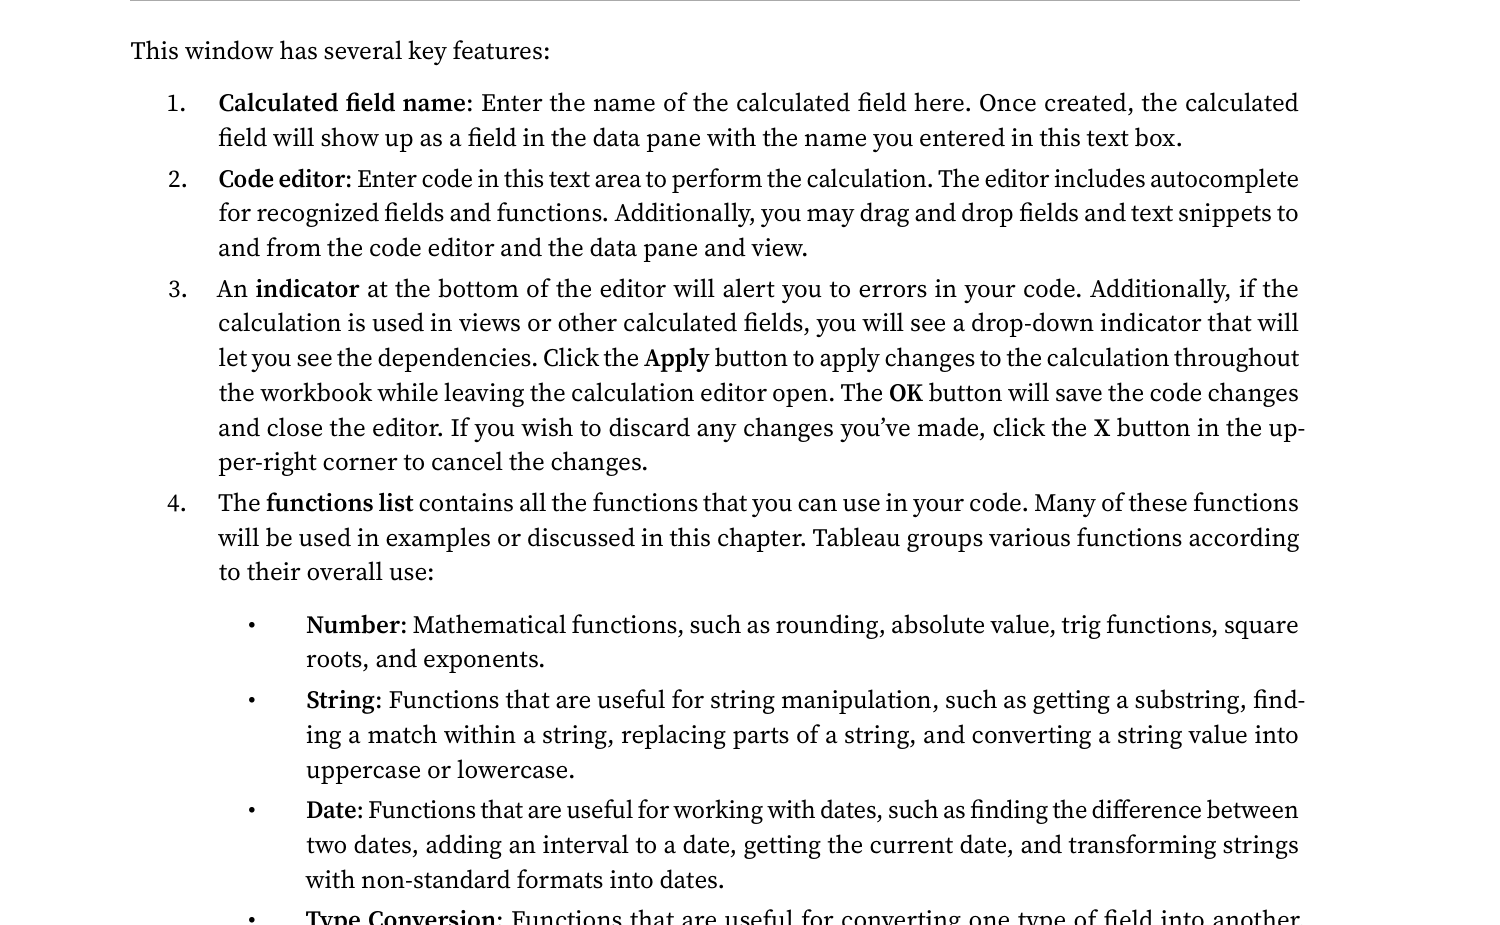
\includegraphics[width=0.9\linewidth]{images/calculated_field_functions.png}
\caption{Cửa sổ Calculated Field --- các thành phần chính gồm: (1) ô nhập tên field, (2) vùng soạn code, (3) indicator lỗi, và (4) danh sách hàm phân loại theo Number, String, Date, Type Conversion...}
\label{fig:calculated_field}
\end{figure}

\noindent Trong phần này, chúng ta sẽ khám phá các hàm preprocessing được tổ chức theo \textbf{kiểu dữ liệu (data type)} --- vì mỗi kiểu có bộ hàm riêng phù hợp với đặc điểm của nó.

% ===================================================================
\section{Data Types trong Tableau}
% ===================================================================

\noindent Khi kết nối với nguồn dữ liệu, Tableau tự động phân tích và gán \textbf{kiểu dữ liệu (data type)} cho từng cột dựa trên nội dung của nó. Mỗi data type được nhận diện thông qua một \textbf{icon đặc trưng} hiển thị bên trái tên field trong Data Pane. Việc hiểu đúng data type cực kỳ quan trọng vì nó quyết định hàm nào có thể áp dụng, loại aggregation nào được phép, và biểu đồ nào Tableau sẽ gợi ý khi bạn drag field vào canvas.

\noindent Tableau hỗ trợ 6 data type cơ bản, được tóm tắt trong bảng sau:

\begin{center}
\renewcommand{\arraystretch}{1.4}
\begin{tabularx}{\linewidth}{c l X X}
\toprule
\textbf{Icon} & \textbf{Data Type} & \textbf{Mô tả} & \textbf{Ví dụ trong Superstore} \\
\midrule
\textbf{Abc} & \textbf{String} & Văn bản --- chuỗi ký tự bất kỳ & \texttt{Customer Name}, \texttt{Product Name}, \texttt{Region} \\
\textbf{\#} & \textbf{Number} & Số --- nguyên hoặc thập phân & \texttt{Sales}, \texttt{Profit}, \texttt{Quantity}, \texttt{Discount} \\
\faIcon{calendar} & \textbf{Date} & Ngày tháng --- chỉ có ngày, không có giờ & \texttt{Order Date}, \texttt{Ship Date} \\
\faIcon{calendar}\faIcon{clock} & \textbf{Date \& Time} & Ngày tháng kèm giờ phút giây & Dấu thời gian giao dịch hệ thống \\
\textbf{T|F} & \textbf{Boolean} & Nhị phân --- chỉ có True hoặc False & Kết quả so sánh, điều kiện lọc \\
\faIcon{globe} & \textbf{Geographic} & Địa lý --- Tableau tự nhận diện để vẽ bản đồ & \texttt{Country}, \texttt{State}, \texttt{City}, \texttt{Postal Code} \\
\bottomrule
\end{tabularx}
\end{center}

\begin{figure}[H]
\centering
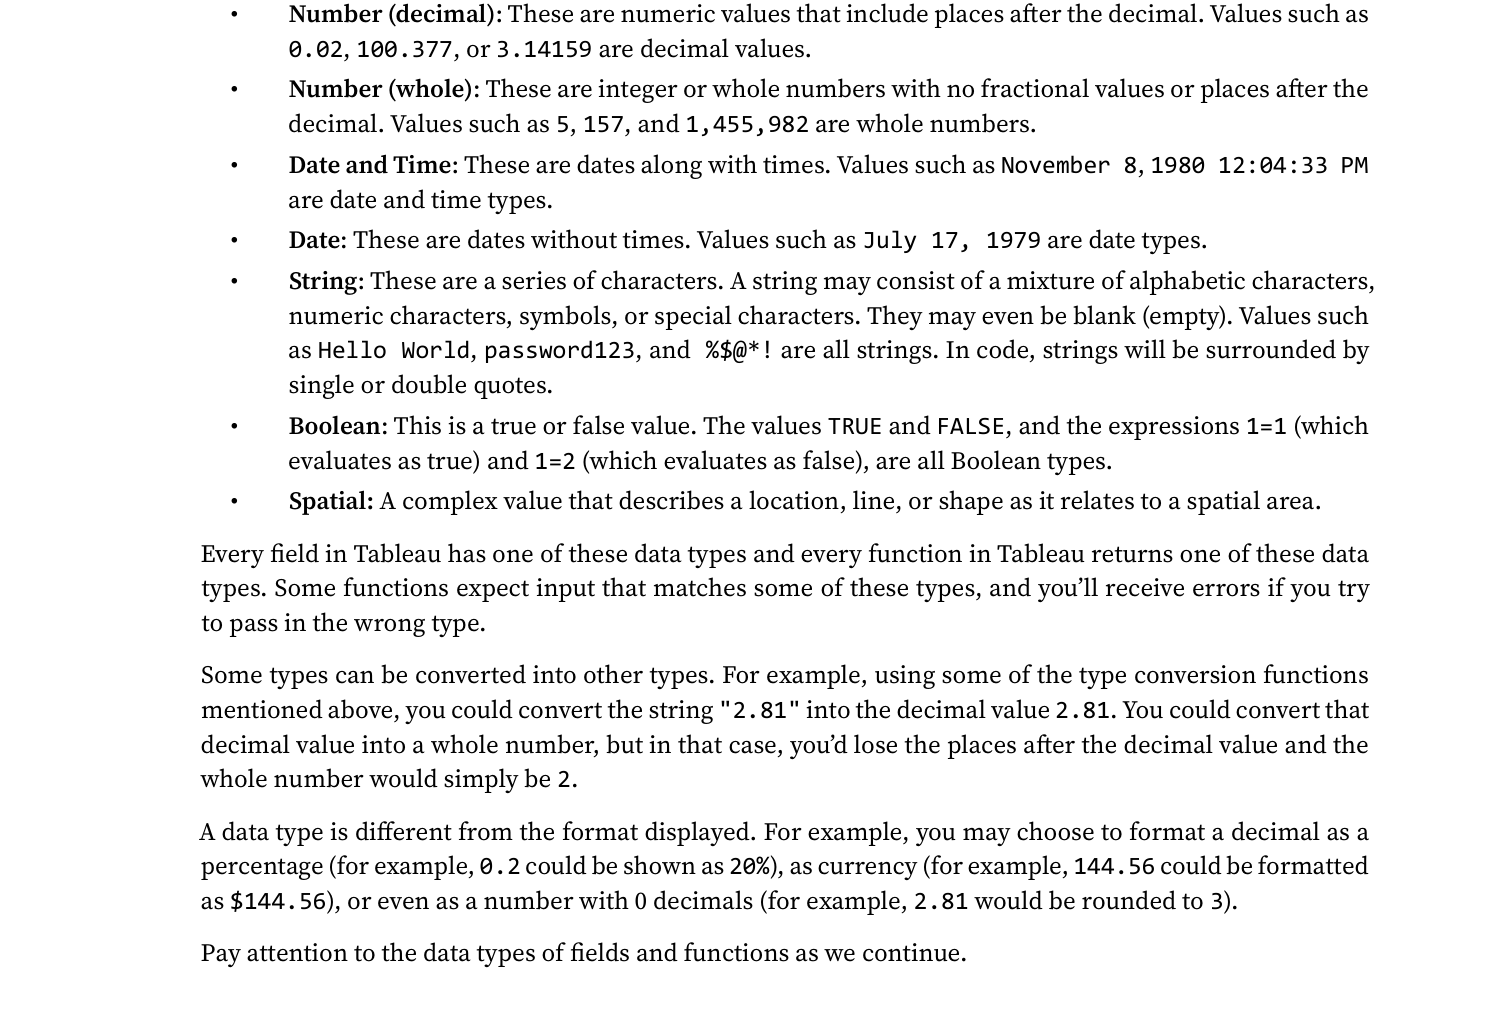
\includegraphics[width=0.9\linewidth]{images/data_types_list.png}
\caption{Data Types trong Tableau --- giải thích chi tiết các kiểu dữ liệu: Number (decimal và whole), Date and Time, Date, String, Boolean, và Spatial.}
\label{fig:data_types}
\end{figure}

\begin{notebox}
\textbf{Tableau có thể nhận sai data type.} Tableau nhận diện data type dựa trên mẫu dữ liệu trong file, nhưng đôi khi mắc lỗi. Trường hợp phổ biến nhất là cột \texttt{Order Date} trong file CSV bị lưu với định dạng không chuẩn (\texttt{"15/1/2024"} thay vì \texttt{"2024-01-15"}) khiến Tableau nhận nhầm thành String --- mọi hàm ngày tháng sẽ thất bại.

\noindent \textbf{Cách kiểm tra nhanh:} Nhìn vào icon bên trái tên field trong Data Pane. Nếu thấy \textbf{Abc} cho một cột mà bạn biết là ngày tháng hoặc số, đó là dấu hiệu dữ liệu cần được chuyển đổi kiểu trước khi phân tích.
\end{notebox}

% ===================================================================
\section{Preprocessing Functions theo Data Type}
% ===================================================================

\noindent Tableau cung cấp hàng chục hàm preprocessing, được phân loại theo data type mà chúng xử lý. Trong thực tế, phần lớn các vấn đề tiền xử lý dữ liệu đều rơi vào 4 nhóm: \textbf{String}, \textbf{Number}, \textbf{Date}, và \textbf{Type Conversion}. Chúng ta sẽ đi sâu vào từng nhóm với bối cảnh thực tế và ví dụ cụ thể từ dataset Superstore.

% -------------------------------------------------------------------
\subsection{String Functions --- Xử lý văn bản}
% -------------------------------------------------------------------

\noindent Khi làm việc với dữ liệu thực tế, các trường văn bản thường là nguồn gốc của nhiều lỗi tinh vi nhất. Một cột \texttt{Customer Name} xuất từ hệ thống CRM có thể chứa khoảng trắng thừa ở đầu và cuối (do nhập liệu), viết hoa viết thường không nhất quán, hoặc thậm chí có ký tự đặc biệt không mong muốn. Những lỗi này không gây ra thông báo lỗi --- Tableau vẫn chạy bình thường --- nhưng kết quả phân tích sẽ sai: cùng một khách hàng nhưng bị đếm thành nhiều người khác nhau, filter không hoạt động đúng, hay group by ra kết quả thiếu.

\noindent Tableau cung cấp một bộ hàm String phong phú để giải quyết các vấn đề này. Dưới đây là các hàm thực dụng nhất mà một nhà phân tích dữ liệu cần nắm:

\begin{itemize}
    \item \textbf{\texttt{UPPER(string)} và \texttt{LOWER(string)}:} Chuyển đổi toàn bộ chuỗi sang chữ HOA hoặc chữ thường. Đây là thao tác chuẩn hóa đầu tiên khi cần so sánh hoặc nhóm dữ liệu văn bản --- \texttt{"Furniture"} và \texttt{"furniture"} là hai giá trị khác nhau trong Tableau, nhưng sau khi áp dụng \texttt{LOWER()} chúng sẽ hợp nhất thành một nhóm duy nhất.

    \item \textbf{\texttt{TRIM(string)}:} Xóa khoảng trắng ở \textbf{đầu và cuối} chuỗi --- không xóa khoảng trắng ở giữa. Đây là một trong những hàm quan trọng nhất vì khoảng trắng thừa hoàn toàn vô hình khi nhìn bằng mắt, nhưng khiến \texttt{"Hà Nội"} và \texttt{" Hà Nội"} trở thành hai chuỗi khác nhau và filter sẽ không khớp.

    \item \textbf{\texttt{LEFT(string, number)} và \texttt{RIGHT(string, number)}:} Trích xuất \texttt{n} ký tự từ bên trái hoặc bên phải của chuỗi. Ứng dụng phổ biến: trích xuất mã tỉnh/thành từ \texttt{"HN-001"} bằng \texttt{LEFT([City Code], 2)} để lấy \texttt{"HN"}.

    \item \textbf{\texttt{MID(string, start, length)}:} Trích xuất một đoạn con từ giữa chuỗi, bắt đầu từ vị trí \texttt{start} (1-indexed) với độ dài \texttt{length} ký tự. Ví dụ \texttt{"US-2024-00123"} --- ta có thể dùng \texttt{MID([Order ID], 4, 4)} để lấy năm \texttt{"2024"}.

    \item \textbf{\texttt{REPLACE(string, old, new)}:} Tìm và thay thế tất cả các lần xuất hiện của \texttt{old} bằng \texttt{new}. Ví dụ: \texttt{REPLACE([Phone], "-", "")} để xóa dấu gạch trong số điện thoại \texttt{"090-123-4567"} $\rightarrow$ \texttt{"0901234567"}.

    \item \textbf{\texttt{CONTAINS(string, substring)}:} Kiểm tra xem chuỗi có chứa chuỗi con không, trả về \texttt{True} hoặc \texttt{False}. Ví dụ: \texttt{CONTAINS([Product Name], "Chair")} trả về True cho tất cả sản phẩm có chữ ``Chair'' trong tên.

    \item \textbf{\texttt{LEN(string)}:} Đếm tổng số ký tự trong chuỗi. Thường dùng để kiểm tra dữ liệu: nếu mã sản phẩm phải có đúng 8 ký tự, \texttt{LEN([Product ID]) != 8} sẽ phát hiện các mã bị lỗi.

    \item \textbf{\texttt{SPLIT(string, delimiter, token\_number)}:} Tách chuỗi thành các phần dựa trên ký tự phân cách và lấy phần thứ \texttt{token\_number}. Ví dụ \texttt{SPLIT("Furniture/Bookcases", "/", 2)} trả về \texttt{"Bookcases"}.

    \item \textbf{Toán tử nối chuỗi \texttt{+}:} Dấu cộng \texttt{+} dùng để \textbf{ghép nối (concatenate)} các chuỗi. Ví dụ: \texttt{[First Name] + " " + [Last Name]} tạo ra \texttt{"Claire Gute"}. Lưu ý: \textbf{phải thêm khoảng trắng thủ công} vào công thức (\texttt{+ " " +}).

    \item \textbf{\texttt{STARTSWITH(string, substring)}:} Kiểm tra xem chuỗi có \textbf{bắt đầu} bằng chuỗi con không, trả về \texttt{True/False}. \texttt{STARTSWITH([Order ID], "US")} trả về True cho tất cả đơn hàng có mã bắt đầu bằng ``US''.

    \item \textbf{\texttt{ENDSWITH(string, substring)}:} Kiểm tra xem chuỗi có \textbf{kết thúc} bằng chuỗi con không. \texttt{ENDSWITH([File Name], ".csv")} trả về True cho các file CSV.

    \item \textbf{\texttt{FIND(string, substring, [start])}:} Tìm vị trí của chuỗi con trong chuỗi --- trả về số thứ tự ký tự (1-indexed), hoặc \textbf{0 nếu không tìm thấy}. Ví dụ: \texttt{FIND("CA-2024-01", "-")} = 3.

    \item \textbf{\texttt{LTRIM(string)} và \texttt{RTRIM(string)}:} Xóa khoảng trắng \textbf{chỉ bên trái} (\texttt{LTRIM}) hoặc \textbf{chỉ bên phải} (\texttt{RTRIM}) --- chi tiết hơn \texttt{TRIM()} vốn xóa cả 2 phía.
\end{itemize}

\noindent \textbf{Ví dụ tổng hợp --- Chuẩn hóa tên khách hàng:}

\noindent Giả sử trường \texttt{Customer Name} trong Superstore có giá trị lộn xộn như \texttt{"~~CLAIRE GUTE~~"} (thừa khoảng trắng, toàn chữ hoa). Chúng ta tạo một Calculated Field mới tên \texttt{[Customer Name Cleaned]}:

\begin{aivncodebox}[]
\begin{lstlisting}
// Xóa khoảng trắng dư + chuyển về chữ thường để chuẩn hóa so sánh
LOWER(TRIM([Customer Name]))

// Kết quả: "claire gute"
\end{lstlisting}
\end{aivncodebox}

\noindent Hoặc nếu muốn kiểm tra nhanh tên nào còn khoảng trắng thừa (để lọc ra dữ liệu lỗi):

\begin{aivncodebox}[]
\begin{lstlisting}
// True = có khoảng trắng thừa ở đầu hoặc cuối
LEN([Customer Name]) != LEN(TRIM([Customer Name]))

// Kết quả: True / False
\end{lstlisting}
\end{aivncodebox}

\begin{figure}[H]
\centering
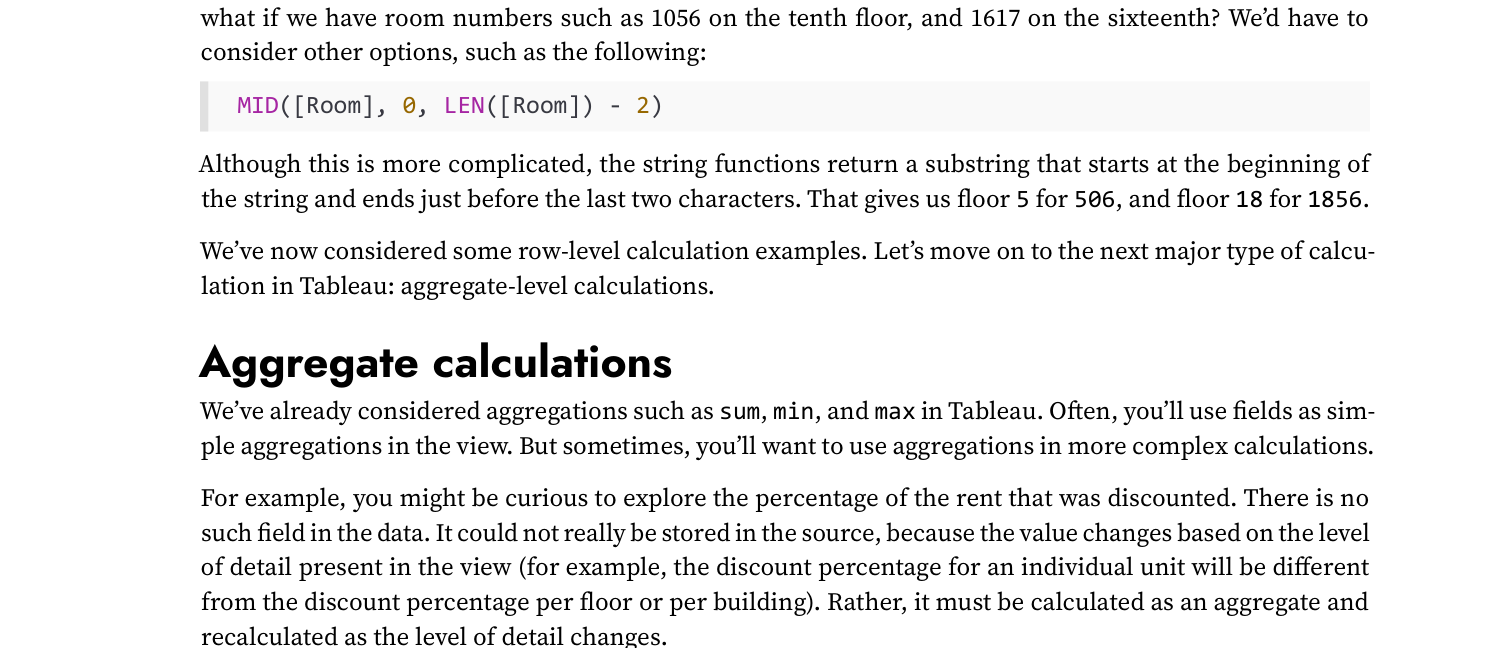
\includegraphics[width=0.9\linewidth]{images/string_functions_example.png}
\caption{Ví dụ String Functions --- sử dụng \texttt{MID} và \texttt{LEN} để trích xuất thông tin từ chuỗi. Mã màu cú pháp giúp phân biệt tên hàm (xanh), tên field (cam), và hằng số (tím).}
\label{fig:string_functions}
\end{figure}

\begin{tipbox}{Tableau không có hàm PROPER()}
Python có \texttt{str.title()} và Excel có \texttt{PROPER()} để viết hoa chữ cái đầu mỗi từ, nhưng Tableau không có hàm tương đương sẵn có.

\noindent Workaround đơn giản cho tên một từ: \texttt{UPPER(LEFT([Name], 1)) + LOWER(MID([Name], 2, LEN([Name])))}

\noindent Tuy nhiên với tên nhiều từ (như tên người), workaround này chỉ viết hoa được từ đầu tiên. Đối với trường hợp này, tốt hơn nên xử lý bằng Python trước khi import vào Tableau.
\end{tipbox}

% -------------------------------------------------------------------
\subsection{Number Functions --- Xử lý số}
% -------------------------------------------------------------------

\noindent Dữ liệu số trong Tableau ít gặp lỗi về kiểu hơn String, nhưng vẫn cần xử lý trong nhiều tình huống: làm tròn để hiển thị gọn gàng, lấy trị tuyệt đối khi chỉ quan tâm độ lớn, hay xử lý giá trị NULL khiến mọi phép tính đều trả về NULL thay vì giá trị thực.

\noindent Trong dataset Superstore, trường \texttt{Profit} là ví dụ điển hình --- nó có thể mang giá trị âm khi đơn hàng bị lỗ, và trường \texttt{Discount} thường là số thập phân (0.1, 0.2, ...) cần làm tròn khi hiển thị. Dưới đây là các hàm Number thực dụng nhất:

\begin{itemize}
    \item \textbf{\texttt{ROUND(number, decimal\_places)}:} Làm tròn đến số chữ số thập phân chỉ định. \texttt{ROUND([Sales], 2)} làm tròn doanh thu đến 2 chữ số thập phân. Khi \texttt{decimal\_places = 0}, hàm làm tròn về số nguyên gần nhất. Khi \texttt{decimal\_places} là số âm, hàm làm tròn về hàng chục, hàng trăm... ví dụ \texttt{ROUND(1234, -2)} = 1200.

    \item \textbf{\texttt{CEILING(number)} và \texttt{FLOOR(number)}:} Hai hàm làm tròn ``lệch'' --- \texttt{CEILING()} luôn làm tròn \textbf{lên} đến số nguyên tiếp theo (ví dụ \texttt{CEILING(3.2)} = 4), còn \texttt{FLOOR()} luôn làm tròn \textbf{xuống} (ví dụ \texttt{FLOOR(3.8)} = 3). Hữu ích trong các bài toán phân nhóm hay làm tròn giá vé, chi phí vận chuyển.

    \item \textbf{\texttt{ABS(number)}:} Trả về giá trị tuyệt đối --- bỏ dấu âm. \texttt{ABS([Profit])} cho biết độ lớn của lãi/lỗ bất kể chiều hướng. Thường dùng: \texttt{ABS([Actual] - [Target])}.

    \item \textbf{\texttt{ZN(expression)}:} Viết tắt của \textbf{``Zero if Null''} --- nếu biểu thức trả về NULL thì thay bằng 0, ngược lại giữ nguyên giá trị. Đây là một trong những hàm quan trọng nhất khi làm việc với dữ liệu có missing values, vì trong Tableau bất kỳ phép tính nào có NULL đều trả về NULL: \texttt{NULL + 100 = NULL}, \texttt{NULL * 5 = NULL}.

    \item \textbf{\texttt{POWER(number, exponent)}:} Tính lũy thừa. \texttt{POWER([Sales], 2)} = Sales bình phương. Cần thiết khi tính các chỉ số thống kê hoặc chuẩn hóa dữ liệu.

    \item \textbf{\texttt{SIGN(number)}:} Trả về \textbf{--1} nếu số âm, \textbf{0} nếu bằng 0, \textbf{1} nếu dương. Kết hợp với CASE: \texttt{CASE SIGN([Profit]) WHEN 1 THEN "Lãi" WHEN -1 THEN "Lỗ" ELSE "Hòa vốn" END}.

    \item \textbf{\texttt{DIV(integer1, integer2)}:} Chia nguyên --- trả về phần nguyên của phép chia. \texttt{DIV(7, 2)} = 3 (không phải 3.5). Hữu ích khi tính số lô hàng nguyên: \texttt{DIV([Quantity], [Batch Size])}.
\end{itemize}

\noindent \textbf{Ví dụ tổng hợp --- Phân loại đơn hàng theo lợi nhuận:}

\begin{aivncodebox}[]
\begin{lstlisting}
// Phân loại đơn hàng: Lãi, Huề vốn, hoặc Lỗ
IF [Profit] > 0 THEN "Profitable"
ELSEIF [Profit] = 0 THEN "Break-even"
ELSE "Loss"
END

// Kết quả: "Profitable" / "Break-even" / "Loss" cho từng dòng
\end{lstlisting}
\end{aivncodebox}

\noindent Và tính \textbf{tỷ suất lợi nhuận (profit margin)} một cách an toàn, tránh lỗi chia cho 0:

\begin{aivncodebox}[]
\begin{lstlisting}
// ZN đảm bảo khi Sales = NULL thì kết quả = 0 thay vì NULL
ZN([Profit]) / ZN([Sales])

// Hoặc viết cẩn thận hơn để tránh lỗi chia cho 0:
IF ZN([Sales]) = 0 THEN 0
ELSE [Profit] / [Sales]
END
\end{lstlisting}
\end{aivncodebox}

\begin{warningbox}{NULL trong Tableau $\neq$ 0}
Đây là một trong những điểm gây nhầm lẫn phổ biến nhất. Trong Tableau, NULL không phải là 0 --- nó là ``không có dữ liệu''. Mọi phép tính số học với NULL đều trả về NULL, không phải một số.

\noindent Ví dụ thực tế: Nếu một khách hàng chưa có đơn hàng nào trong tháng, trường \texttt{Sales} của họ là NULL (không phải 0). \texttt{SUM(NULL, 50, 30)} = 80 --- hàm SUM bỏ qua NULL. Nhưng \texttt{NULL / 100} = NULL --- phép chia thất bại. Luôn dùng \texttt{ZN()} trước khi thực hiện phép chia để đảm bảo an toàn.
\end{warningbox}

% -------------------------------------------------------------------
\subsection{Date Functions --- Xử lý ngày tháng}
% -------------------------------------------------------------------

\noindent Phân tích theo thời gian là một trong những yêu cầu phổ biến nhất trong Business Intelligence. Với dataset Superstore có hai trường date là \texttt{Order Date} và \texttt{Ship Date}, chúng ta cần khả năng: tách năm/quý/tháng để nhóm dữ liệu, tính khoảng cách giữa ngày đặt hàng và ngày giao hàng, hay lọc ra các đơn hàng trong 30 ngày gần nhất so với ngày hôm nay.

\noindent Trước khi bắt đầu, cần hiểu khái niệm quan trọng nhất trong Date Functions --- tham số \textbf{\texttt{date\_part}}. Đây là một chuỗi chỉ định \textbf{đơn vị thời gian} mà hàm sẽ làm việc với:

\begin{center}
\renewcommand{\arraystretch}{1.4}
\begin{tabularx}{\linewidth}{l l X}
\toprule
\textbf{Giá trị \texttt{date\_part}} & \textbf{Ý nghĩa} & \textbf{Kết quả (ví dụ với 15/03/2024)} \\
\midrule
\texttt{'year'} & Năm & 2024 \\
\texttt{'quarter'} & Quý trong năm & 1 (Q1: tháng 1--3) \\
\texttt{'month'} & Tháng trong năm & 3 \\
\texttt{'day'} & Ngày trong tháng & 15 \\
\texttt{'weekday'} & Thứ trong tuần & 6 (6 = Thứ Sáu, ISO) \\
\texttt{'hour'} & Giờ (chỉ dùng với Date \& Time) & 0--23 \\
\bottomrule
\end{tabularx}
\end{center}

\noindent Các hàm Date thực dụng nhất trong phân tích dữ liệu bán hàng:

\begin{itemize}
    \item \textbf{\texttt{YEAR(date)}, \texttt{MONTH(date)}, \texttt{DAY(date)}:} Ba hàm đơn giản nhất để trích xuất năm, tháng, ngày từ một trường Date. \texttt{YEAR([Order Date])} trả về số nguyên như 2021, 2022... Đây là cách nhanh nhất để tạo các trường phụ trợ phục vụ nhóm dữ liệu theo thời gian.

    \item \textbf{\texttt{DATEPART(date\_part, date)}:} Tổng quát hơn \texttt{YEAR/MONTH/DAY} --- có thể lấy bất kỳ đơn vị thời gian nào. \texttt{DATEPART('quarter', [Order Date])} trả về 1, 2, 3, hoặc 4. Kết quả là \textbf{số nguyên}, phù hợp cho tính toán.

    \item \textbf{\texttt{DATENAME(date\_part, date)}:} Tương tự \texttt{DATEPART} nhưng trả về \textbf{tên dạng chuỗi}. \texttt{DATENAME('month', [Order Date])} trả về \texttt{"January"}, \texttt{"February"}... Hữu ích khi muốn hiển thị nhãn thân thiện trên biểu đồ.

    \item \textbf{\texttt{DATEDIFF(date\_part, start\_date, end\_date)}:} Tính \textbf{khoảng cách} giữa hai ngày. \texttt{DATEDIFF('day', [Order Date], [Ship Date])} cho biết mất bao nhiêu ngày để giao hàng.

    \item \textbf{\texttt{DATEADD(date\_part, interval, date)}:} Cộng (hoặc trừ nếu \texttt{interval} âm) một khoảng thời gian vào một ngày. \texttt{DATEADD('month', 3, [Order Date])} trả về ngày 3 tháng sau ngày đặt hàng.

    \item \textbf{\texttt{TODAY()}:} Trả về ngày hôm nay (không có giờ). Thường kết hợp với \texttt{DATEDIFF} để tạo filter động.

    \item \textbf{\texttt{DATETRUNC(date\_part, date)}:} ``Cắt'' ngày về \textbf{đầu kỳ} tương ứng. \texttt{DATETRUNC('month', \#2024-03-15\#)} = \textbf{1/3/2024}; \texttt{DATETRUNC('quarter', \#2024-03-15\#)} = \textbf{1/1/2024}. Cực kỳ hữu ích khi cần so sánh các kỳ với nhau.

    \item \textbf{\texttt{NOW()}:} Trả về \textbf{ngày và giờ hiện tại} (Date \& Time) --- khác với \texttt{TODAY()} chỉ trả về ngày. Lưu ý: \texttt{NOW()} tính theo múi giờ của máy chủ Tableau, không phải browser người dùng.

    \item \textbf{\texttt{QUARTER(date)} và \texttt{WEEK(date)}:} Shorthand nhanh --- \texttt{QUARTER([Order Date])} trả về 1--4; \texttt{WEEK([Order Date])} trả về số tuần trong năm (1--52/53).

    \item \textbf{\texttt{MAKEDATE(year, month, day)}:} Tạo một giá trị Date từ 3 số nguyên riêng lẻ. \texttt{MAKEDATE(2024, 3, 15)} tạo ngày 15/3/2024. Hữu ích khi dữ liệu lưu riêng năm, tháng, ngày trong 3 cột Number.

    \item \textbf{\texttt{DATEPARSE(format, string)}:} Chuyển đổi một \textbf{chuỗi} có định dạng đặc biệt thành kiểu Date. Ví dụ:
\end{itemize}

\begin{aivncodebox}[]
\begin{lstlisting}
DATEPARSE("MMMM,d,yy", "September,4,12")
// Kết quả: 9/4/2012 (ngày tháng năm theo ISO)
\end{lstlisting}
\end{aivncodebox}

\noindent Các định dạng phổ biến: \texttt{yyyy} = năm 4 chữ số, \texttt{MM} = tháng 2 chữ số, \texttt{dd} = ngày 2 chữ số, \texttt{MMMM} = tên tháng đầy đủ, \texttt{MMM} = tên tháng viết tắt. Chuỗi format phải \textbf{khớp chính xác} với cấu trúc của chuỗi ngày.

\noindent \textbf{Ví dụ tổng hợp --- Phân tích thời gian giao hàng:}

\begin{aivncodebox}[]
\begin{lstlisting}
// Tính số ngày giao hàng (từ Order Date đến Ship Date)
DATEDIFF('day', [Order Date], [Ship Date])
// Kết quả: 2, 3, 5... (số nguyên)

// Phân loại tốc độ giao hàng
IF DATEDIFF('day', [Order Date], [Ship Date]) <= 2
THEN "Fast"
ELSEIF DATEDIFF('day', [Order Date], [Ship Date]) <= 5
THEN "Normal (3-5 days)"
ELSE "Slow (>5 days)"
END

// Lọc đơn hàng trong 365 ngày gần nhất
DATEDIFF('day', [Order Date], TODAY()) <= 365
// Kết quả: True / False — dùng làm filter condition
\end{lstlisting}
\end{aivncodebox}

\begin{tipbox}{DATEPART vs DATENAME: khi nào dùng cái nào?}
\begin{itemize}[nosep]
    \item Dùng \textbf{\texttt{DATEPART('month', ...)}} $\rightarrow$ kết quả là số \texttt{1, 2, ..., 12} $\rightarrow$ khi cần \textbf{tính toán} (so sánh, cộng trừ)
    \item Dùng \textbf{\texttt{DATENAME('month', ...)}} $\rightarrow$ kết quả là \texttt{"January", "February", ...} $\rightarrow$ khi cần \textbf{hiển thị nhãn} trên trục X
\end{itemize}
\noindent Lưu ý: kết quả của \texttt{DATENAME} sẽ sắp xếp theo bảng chữ cái (April, August, December...) thay vì theo thứ tự tháng. Để sắp xếp đúng, hãy dùng thêm \texttt{DATEPART} làm trường sắp xếp phụ trợ (Sort Field).
\end{tipbox}

% -------------------------------------------------------------------
\subsection{Ad-hoc Calculations và xử lý giá trị NULL}
% -------------------------------------------------------------------

\noindent Ngoài việc tạo Calculated Field đầy đủ qua menu \textbf{Analysis $\rightarrow$ Create Calculated Field...}, Tableau còn hỗ trợ một cách tạo công thức nhanh hơn gọi là \textbf{Ad-hoc Calculation}. Phương pháp này cho phép nhập công thức \textbf{trực tiếp trên Columns shelf, Rows shelf, hoặc thẻ Marks} mà không cần đặt tên hay lưu lại.

\noindent \textbf{Cách tạo Ad-hoc Calculation:}
\begin{enumerate}[nosep]
    \item Kéo field \texttt{Profit} vào Columns shelf. Tableau hiển thị \texttt{SUM([Profit])}.
    \item Nhấp đúp vào pill \texttt{SUM([Profit])} trên Columns shelf --- một ô nhập công thức nhỏ xuất hiện.
    \item Sửa thành \texttt{SUM([Profit])/SUM([Sales])} và nhấn \textbf{Enter}. Tableau tính và hiển thị kết quả ngay lập tức.
    \item Nếu muốn lưu lại: kéo pill từ shelf vào \textbf{Data Pane}, Tableau sẽ yêu cầu đặt tên cho Calculated Field.
\end{enumerate}

\noindent Tableau có hệ thống \textbf{mã màu cú pháp} trong Formula Editor:

\begin{center}
\renewcommand{\arraystretch}{1.4}
\begin{tabularx}{\linewidth}{l X}
\toprule
\textbf{Màu/kiểu chữ} & \textbf{Ý nghĩa} \\
\midrule
\textbf{Chữ đỏ} (gạch chân) & Lỗi cú pháp --- di chuột lên để xem gợi ý sửa \\
\texttt{// chữ màu xám} & Comment --- không ảnh hưởng tính toán \\
\textbf{[chữ màu cam]} & Tên field --- cần bao bằng dấu \texttt{[]} \\
\textbf{chữ màu xanh} & Tên hàm (function) \\
\textbf{[chữ màu tím]} & Parameters \\
\textbf{chữ in đậm} & Phép tính được aggregate \\
chữ không in đậm & Phép tính ở mức row-level \\
\bottomrule
\end{tabularx}
\end{center}

\noindent \textbf{Xử lý giá trị NULL với \texttt{ZN()}:}

\noindent Khi kết hợp hoặc trộn lẫn nhiều nguồn dữ liệu, một số ô có thể không có giá trị (NULL). Trong Tableau, \texttt{NULL + bất kì số nào = NULL} --- nghĩa là một giá trị NULL duy nhất sẽ làm cho toàn bộ kết quả là NULL.

\noindent \textbf{Hàm \texttt{ZN(expression)}} (Zero-if-Null) giải quyết vấn đề này:

\begin{aivncodebox}[]
\begin{lstlisting}
// Không an toàn: nếu Discount là NULL, kết quả sẽ là NULL
[Sales] * [Discount]

// An toàn: ZN thay NULL bằng 0 trước
ZN([Sales]) * ZN([Discount])
\end{lstlisting}
\end{aivncodebox}

\noindent Lưu ý: \texttt{ZN} chỉ dùng đối với số (Number) --- thay NULL số bằng 0 thường hợp lý (không có Discount có nghĩa Discount = 0\%), nhưng cần cân nhắc kỹ trong ngữ cảnh cụ thể.

% -------------------------------------------------------------------
\subsection{Type Conversion Functions --- Chuyển đổi kiểu dữ liệu}
% -------------------------------------------------------------------

\noindent Một trong những vấn đề phổ biến nhất khi import dữ liệu vào Tableau là \textbf{kiểu dữ liệu bị nhận sai}. Nguyên nhân thường gặp: file CSV có cột số nhưng chứa ký tự không phải số (dấu phẩy \texttt{"1,234.56"}, đơn vị tiền tệ \texttt{"\$500"}), cột ngày tháng có định dạng không chuẩn, hoặc Tableau đọc toàn bộ cột là String vì có một vài ô chứa chữ.

\noindent Khi dữ liệu bị nhận sai kiểu, hậu quả rất rõ ràng: không thể tính \texttt{SUM([Revenue])} nếu Revenue là String, không thể dùng \texttt{YEAR([Order Date])} nếu Order Date là String. Type Conversion Functions cho phép chúng ta ép kiểu (cast) dữ liệu sang đúng loại:

\begin{itemize}
    \item \textbf{\texttt{INT(expression)}:} Chuyển đổi sang số nguyên, cắt bỏ phần thập phân (không làm tròn --- \texttt{INT(3.9)} = 3, không phải 4).

    \item \textbf{\texttt{FLOAT(expression)}:} Chuyển đổi sang số thực (có phần thập phân). Phổ biến hơn \texttt{INT} vì giữ được độ chính xác. \texttt{FLOAT("1234.56")} trả về số \texttt{1234.56}.

    \item \textbf{\texttt{STR(expression)}:} Chuyển đổi \textbf{sang String}. Hữu ích khi cần ghép Number vào chuỗi: \texttt{"Order \#" + STR([Order ID])} tạo ra \texttt{"Order \#12345"}.

    \item \textbf{\texttt{DATE(expression)}:} Chuyển đổi String hoặc Number sang kiểu Date. \texttt{DATE("2024-01-15")} trả về ngày 15/1/2024 với đầy đủ khả năng sử dụng các Date Functions.

    \item \textbf{\texttt{DATETIME(expression)}:} Tương tự \texttt{DATE()} nhưng tạo ra giá trị Date \& Time, bao gồm cả giờ phút giây.
\end{itemize}

\noindent \textbf{Ví dụ tổng hợp --- Sửa cột dữ liệu bị nhận sai kiểu:}

\begin{aivncodebox}[]
\begin{lstlisting}
// Trường hợp 1: Cột "Revenue_str" = "1234.56" (String)
// -> Chuyển thành Number để có thể SUM, AVG
FLOAT([Revenue_str])
// Kết quả: 1234.56

// Trường hợp 2: Cột "Order_Date_str" = "2024-01-15" (String)
// -> Chuyển thành Date để dùng YEAR(), DATEDIFF()...
DATE([Order_Date_str])
// Kết quả: 15/01/2024 (Date)

// Trường hợp 3: Tạo label kết hợp số và chữ
"Đơn hàng #" + STR([Order ID]) + " — " + STR([Customer Name])
// Kết quả: "Đơn hàng #12345 — Claire Gute"
\end{lstlisting}
\end{aivncodebox}

\begin{notebox}
\textbf{Nhận biết lỗi kiểu dữ liệu ngay từ đầu ---} Có 3 dấu hiệu rõ ràng:
\begin{enumerate}[nosep]
    \item Field có icon \textbf{Abc} trong Data Pane nhưng bạn biết nó là số hoặc ngày
    \item Tableau báo lỗi \textbf{``Cannot mix aggregate and non-aggregate arguments''} khi bạn cố tính SUM
    \item Tableau không gợi ý \textbf{Line Chart} khi bạn drag một Date field vào Columns
\end{enumerate}
\noindent Bước xử lý chuẩn: tạo Calculated Field mới dùng \texttt{FLOAT()}, \texttt{DATE()}, hay \texttt{INT()} để chuyển đổi, đặt tên rõ ràng (ví dụ \texttt{[Sales (Numeric)]}), rồi sử dụng field mới đó thay cho field gốc.
\end{notebox}

% -------------------------------------------------------------------
\subsection{Logical Functions --- Phân loại và điều kiện hóa dữ liệu}
% -------------------------------------------------------------------

\noindent Nếu String Functions giúp làm sạch dữ liệu và Date Functions giúp phân tích thời gian, thì \textbf{Logical Functions} là trái tim của mọi phân tích dữ liệu có chiều sâu --- chúng cho phép Tableau đưa ra \textbf{quyết định} dựa trên điều kiện, phân loại dữ liệu thành nhóm, và xử lý các trường hợp đặc biệt.

\subsubsection{IF / ELSEIF / ELSE / END --- Điều kiện nhiều nhánh}

\noindent Cú pháp IF là cách phổ biến nhất để phân loại dữ liệu trong Tableau:

\begin{aivncodebox}[]
\begin{lstlisting}
IF <test1> THEN <value1>
ELSEIF <test2> THEN <value2>
...
ELSE <default_value>
END
\end{lstlisting}
\end{aivncodebox}

\begin{itemize}[nosep]
    \item Tableau kiểm tra \textbf{lần lượt} từng điều kiện, trả về giá trị tương ứng với điều kiện đầu tiên là \texttt{True}
    \item \texttt{ELSEIF} và \texttt{ELSE} là tùy chọn --- có thể viết \texttt{IF...THEN...END} đơn giản
    \item Phần \texttt{ELSE} là giá trị mặc định khi không có điều kiện nào khớp --- nếu bỏ qua, kết quả là \texttt{NULL}
\end{itemize}

\noindent \textbf{Ví dụ thực tế --- Phân loại lợi nhuận:}

\begin{aivncodebox}[]
\begin{lstlisting}
// Tạo Calculated Field [Profit Status]
IF [Profit] > 0 THEN "Profitable"
ELSEIF [Profit] = 0 THEN "Break-even"
ELSE "Loss"
END
\end{lstlisting}
\end{aivncodebox}

\noindent \textbf{Ví dụ nâng cao --- Phân loại theo nhiều trường:}

\begin{aivncodebox}[]
\begin{lstlisting}
// Phân loại khách hàng VIP dựa trên cả Sales và Profit
IF SUM([Sales]) > 10000 AND SUM([Profit]) > 1000
THEN "VIP"
ELSEIF SUM([Sales]) > 5000
THEN "Regular"
ELSE "New"
END

// Lưu ý: Khi dùng IF kết hợp aggregate (SUM),
// cả công thức phải ở cấp aggregate
\end{lstlisting}
\end{aivncodebox}

\begin{conceptbox}{IIF (Inline IF)}
\texttt{IIF(<test>, <then>, <else>)} là phiên bản rút gọn của IF cho trường hợp chỉ có 2 nhánh. \texttt{IIF([Profit] > 0, "Lãi", "Lỗ")} tương đương với \texttt{IF [Profit] > 0 THEN "Lãi" ELSE "Lỗ" END}. Dùng khi công thức đơn giản --- nhưng khi cần nhiều điều kiện, IF/ELSEIF dễ đọc hơn nhiều IIF lồng nhau.
\end{conceptbox}

\subsubsection{CASE / WHEN / THEN --- Phân loại theo giá trị cụ thể}

\noindent CASE là lựa chọn tốt hơn IF khi bạn cần so sánh \textbf{một field với nhiều giá trị cụ thể}:

\begin{aivncodebox}[]
\begin{lstlisting}
CASE <expression>
WHEN <value1> THEN <result1>
WHEN <value2> THEN <result2>
...
[ELSE <default>]
END
\end{lstlisting}
\end{aivncodebox}

\noindent \textbf{Ví dụ thực tế --- Dịch tên vùng sang tiếng Việt:}

\begin{aivncodebox}[]
\begin{lstlisting}
CASE [Region]
WHEN "East" THEN "Miền Đông"
WHEN "West" THEN "Miền Tây"
WHEN "North" THEN "Miền Bắc"
WHEN "South" THEN "Miền Nam"
ELSE "Không xác định"
END
\end{lstlisting}
\end{aivncodebox}

\begin{tipbox}{IF vs CASE: khi nào dùng cái nào?}
\renewcommand{\arraystretch}{1.3}
\begin{tabularx}{\linewidth}{X X}
\toprule
\textbf{CASE} & \textbf{IF} \\
\midrule
So sánh \textbf{một field} với nhiều \textbf{giá trị rời rạc} & Kiểm tra \textbf{nhiều điều kiện phức tạp} khác nhau \\
\texttt{[Region] = "East"}, \texttt{[Region] = "West"}... & \texttt{[Sales] > 10000 AND [Profit] > 0}... \\
Cú pháp gọn hơn, dễ đọc hơn & Linh hoạt hơn --- dùng được \texttt{>}, \texttt{<}, \texttt{AND}, \texttt{OR} \\
\bottomrule
\end{tabularx}
\end{tipbox}

\subsubsection{Toán tử logic: AND, OR, NOT}

\noindent Các toán tử này kết hợp nhiều điều kiện vào một biểu thức:

\begin{itemize}
    \item \textbf{\texttt{AND}:} Cả hai điều kiện đều phải \texttt{True}. \texttt{[Sales] > 1000 AND [Profit] > 0} --- chỉ đơn hàng lãi VÀ có doanh thu cao. AND dùng \textbf{short-circuit evaluation}.

    \item \textbf{\texttt{OR}:} Chỉ cần một trong hai điều kiện là \texttt{True}. \texttt{[Region] = "East" OR [Region] = "West"}.

    \item \textbf{\texttt{NOT}:} Đảo ngược kết quả boolean. \texttt{NOT ISNULL([Customer ID])} --- chỉ giữ lại các dòng có Customer ID.
\end{itemize}

\begin{aivncodebox}[]
\begin{lstlisting}
// Ví dụ kết hợp: đơn hàng cần chú ý
// (Lỗ lớn HOẶC chiết khấu cao) VÀ không phải khách VIP
(SUM([Profit]) < -500 OR SUM([Discount]) > 0.3)
AND NOT ([Customer Segment] = "VIP")
\end{lstlisting}
\end{aivncodebox}

\subsubsection{Xử lý NULL: ISNULL, IFNULL và ZN}

\noindent Ba hàm xử lý NULL trong Tableau, mỗi hàm phục vụ mục đích khác nhau:

\begin{center}
\renewcommand{\arraystretch}{1.4}
\begin{tabularx}{\linewidth}{l l l X}
\toprule
\textbf{Hàm} & \textbf{Cú pháp} & \textbf{Trả về} & \textbf{Dùng khi} \\
\midrule
\textbf{\texttt{ISNULL}} & \texttt{ISNULL(expr)} & \texttt{True/False} & Cần \textbf{kiểm tra} xem field có NULL không \\
\textbf{\texttt{IFNULL}} & \texttt{IFNULL(e1, e2)} & Giá trị e1 hoặc e2 & Cần \textbf{thay thế NULL bằng giá trị bất kỳ} \\
\textbf{\texttt{ZN}} & \texttt{ZN(expr)} & Giá trị hoặc \textbf{0} & Cần \textbf{thay NULL bằng 0} cho phép tính số \\
\bottomrule
\end{tabularx}
\end{center}

\begin{aivncodebox}[]
\begin{lstlisting}
// ISNULL — Phát hiện dữ liệu thiếu
ISNULL([Customer ID])
// Kết quả: True cho các dòng chưa có Customer ID

// IFNULL — Thay NULL bằng giá trị mặc định có nghĩa
IFNULL([Assigned Region], "Chưa phân vùng")
// Kết quả: Chuỗi thực hoặc "Chưa phân vùng"

// ZN — Đảm bảo an toàn cho phép tính số
ZN([Discount]) * ZN([Sales])
// Kết quả: Nếu NULL -> kết quả là 0, không phải NULL
\end{lstlisting}
\end{aivncodebox}

\begin{notebox}
\textbf{IFNULL vs ZN vs ISNULL:}
\begin{itemize}[nosep]
    \item \texttt{ISNULL} chỉ \textbf{phát hiện} (trả Boolean), không thay thế
    \item \texttt{IFNULL} thay NULL bằng \textbf{bất kỳ giá trị nào} (String, Number, Date...)
    \item \texttt{ZN} chỉ thay bằng \textbf{0} --- ngắn gọn nhưng chỉ dùng cho Number
    \item Với String: dùng \texttt{IFNULL([Field], "N/A")} thay vì ZN
    \item Với Number: có thể dùng cả \texttt{IFNULL([Field], 0)} hoặc \texttt{ZN([Field])}
\end{itemize}
\end{notebox}

\subsubsection{IN --- So sánh với tập giá trị}

\noindent \texttt{IN} kiểm tra xem một giá trị có nằm trong một danh sách hay không --- ngắn gọn hơn nhiều \texttt{OR} liên tiếp:

\begin{aivncodebox}[]
\begin{lstlisting}
// Thay vì:
[Region] = "East" OR [Region] = "West" OR [Region] = "Central"

// Dùng IN:
[Region] IN ("East", "West", "Central")
// Kết quả: True nếu Region bằng bất kỳ giá trị nào trong danh sách
\end{lstlisting}
\end{aivncodebox}

\noindent \texttt{IN} cũng dùng được với Sets trong Tableau: \texttt{[Customer] IN [Top 10 Customers Set]}.

% ===================================================================
\section{Bảng tổng hợp --- Quick Reference}
% ===================================================================

\noindent Bảng dưới đây tóm tắt toàn bộ các hàm đã học, sắp xếp theo vấn đề thực tế mà bạn có thể gặp:

\begin{center}
\renewcommand{\arraystretch}{1.3}
\small
\begin{tabularx}{\linewidth}{l X l X}
\toprule
\textbf{Data Type} & \textbf{Vấn đề thực tế} & \textbf{Hàm xử lý} & \textbf{Ví dụ nhanh} \\
\midrule
\textbf{String} & Khoảng trắng thừa & \texttt{TRIM()}, \texttt{LTRIM()}, \texttt{RTRIM()} & \texttt{TRIM([Name])} \\
\textbf{String} & Hoa/thường không nhất quán & \texttt{UPPER()}, \texttt{LOWER()} & \texttt{LOWER([Region])} \\
\textbf{String} & Trích xuất một phần & \texttt{LEFT()}, \texttt{RIGHT()}, \texttt{MID()} & \texttt{LEFT([Code], 3)} \\
\textbf{String} & Thay thế ký tự lạ & \texttt{REPLACE()} & \texttt{REPLACE([Phone], "-", "")} \\
\textbf{String} & Kiểm tra chuỗi con & \texttt{CONTAINS()}, \texttt{STARTSWITH()} & \texttt{STARTSWITH([ID], "US")} \\
\textbf{String} & Tìm vị trí chuỗi con & \texttt{FIND()} & \texttt{FIND([Code], "-")} \\
\midrule
\textbf{Number} & Làm tròn & \texttt{ROUND()} & \texttt{ROUND([Sales], 2)} \\
\textbf{Number} & Giá trị NULL & \texttt{ZN()} & \texttt{ZN([Profit])} \\
\textbf{Number} & Trị tuyệt đối & \texttt{ABS()} & \texttt{ABS([Profit])} \\
\textbf{Number} & Hướng âm/dương & \texttt{SIGN()} & \texttt{SIGN([Profit])} \\
\midrule
\textbf{Date} & Nhóm theo năm/quý/tháng & \texttt{YEAR()}, \texttt{DATEPART()} & \texttt{QUARTER([Date])} \\
\textbf{Date} & Cắt về đầu kỳ & \texttt{DATETRUNC()} & \texttt{DATETRUNC('month', [Date])} \\
\textbf{Date} & Label thân thiện & \texttt{DATENAME()} & \texttt{DATENAME('month', [Date])} \\
\textbf{Date} & Khoảng cách 2 ngày & \texttt{DATEDIFF()} & \texttt{DATEDIFF('day', [S], [E])} \\
\textbf{Date} & Ngày giờ hiện tại & \texttt{NOW()}, \texttt{TODAY()} & \texttt{TODAY()} \\
\midrule
\textbf{Kiểu sai} & String $\rightarrow$ Number & \texttt{FLOAT()}, \texttt{INT()} & \texttt{FLOAT([Sales\_str])} \\
\textbf{Kiểu sai} & String $\rightarrow$ Date & \texttt{DATE()}, \texttt{DATEPARSE()} & \texttt{DATE([Date\_str])} \\
\textbf{Kiểu sai} & Number $\rightarrow$ String & \texttt{STR()} & \texttt{"ID: " + STR([ID])} \\
\midrule
\textbf{Logic} & Phân loại nhiều nhánh & \texttt{IF/ELSEIF/ELSE/END} & \texttt{IF [P]>0 THEN "Lãi" ...} \\
\textbf{Logic} & Phân loại theo giá trị & \texttt{CASE/WHEN/THEN/END} & \texttt{CASE [Region] WHEN ...} \\
\textbf{Logic} & Kiểm tra NULL & \texttt{ISNULL()} & \texttt{ISNULL([Customer ID])} \\
\textbf{Logic} & Thay NULL bằng default & \texttt{IFNULL()}, \texttt{ZN()} & \texttt{IFNULL([Region], "N/A")} \\
\bottomrule
\end{tabularx}
\end{center}

\vspace{1em}
\noindent \textit{Phần tiếp theo: \textbf{Basic Charts} --- Tạo các loại biểu đồ cơ bản trong Tableau.}

\end{document}
